\section{Pianificazione}
Nella pianificazione, il responsabile suddividerà il lavoro in attività e le assegnerà a ciascun membro del team qbteam.
Lo scopo è quello di mostrare come verrà svolto il lavoro, valutare i progressi nel progetto e anticipare i problemi che potrebbero sorgere preparando così delle soluzioni a tali problemi. 
La pianificazione di progetto è stata organizzata seguendo le scadenze presenti nella sezione Scadenze.
Lo sviluppo del progetto è stato suddiviso nei seguenti 5 macro periodi: 
\begin{itemize}
	\item Analisi;
	\item Progettazione architetturale;
	\item Progettazione di dettaglio e codifica;
	\item Validazione e collaudo;
\end{itemize}
Ogni macro periodo sarò suddiviso a sua volta in altri periodi più brevi in cui verranno elencate le diverse attività che il gruppo qbteam svolgerà.


\subsection{Analisi}

\subsubsection{Periodo 1} 
Dal 15/11/2019 al 29/11/2019\\
In questo periodo, che parte dalla formazione del gruppo e termina con la scelta del capitolato C5, abbiamo affrontato le seguenti tematiche al fine di porre le basi per il lavoro che dovevamo affrontare\\
\begin{itemize}
	\item \textbf{Discussione capitolati:} per prima cosa abbiamo studiato individualmente e in seguito discusso durante gli incontri tutti i capitolati proposti, questo ha posto le basi per la stesura del documento Studio di Fattibilità e ci ha indirizzati verso la scelta del capitolato che avremmo affrontato;
	\item \textbf{Spartizione e studio dei ruoli:} a ogni membro del gruppo è stato assegnato il ruolo che svolgerà nella fase di Analisi;
	\item \textbf{Definizione degli strumenti:} Abbiamo discusso e definito le tecnologie che avremmo usato per affrontare la fase di Analisi;
	\item \textbf{Pianificazione milestone fase di Analisi:} Abbiamo discusso e fissato delle milestone da rispettare per completare la fase di Analisi entro le scadenze imposteci;
\end{itemize}
\subsubsection{Periodo 2} 
Dal 30/11/2019 al 31/12/2019\\
Questo periodo inizia con la scelta definitiva del capitolato C5.\\
Dopo la scelta abbiamo focalizzato le risorse del gruppo sui seguenti punti:
\begin{itemize}
	\item \textbf{Normazione: }Abbiamo definito le regole per la stesura dei documenti e per l'utilizzo delle tecnologie identificate in precedenza;
	\item \textbf{Approfondimento capitolati: }Abbiamo ulteriormente discusso tutti i capitolati in modo da terminare lo studio di fattibilità e focalizzato la nostra analisi su quello scelto in modo da predisporre le basi per l'analisi dei requisiti;
	\item \textbf{Prima definizione dei casi d'uso};
	\item \textbf{Determinazione standard di qualità: }Abbiamo definito le nostre strategie per garantire la qualità di processo e di prodotto;
	\item \textbf{Verifica: }Verifica dell'andamento del team in relazione alle tempistiche e allo svolgimento dei compiti assegnati;
\end{itemize}
\subsubsection{Periodo 3}
 Dal 01/01/2019 al 14/01/2019\\
 Questo periodo si estende fino alla data ultima di consegna per affrontare la revisione dei requisiti a cui il nostro gruppo ha deciso di partecipare.\\
 \begin{itemize}
	\item \textbf{Normazione: }Ulteriori approfondimenti alle regole per la stesura dei documenti e per l'utilizzo delle tecnologie;
	\item \textbf{Approfondimento delle tecnologie: }Abbiamo ampliato le nostre conoscenze sulle tecnologie richieste dal capitolato per essere svolto;
	\item \textbf{Analisi dei requisiti: } Studio dei requisiti e raffinazione dei casi d'uso;
	\item \textbf{Pianificazione attività: }Pianificazione del lavoro da svolgere nelle fasi successive a quella di analisi;
	\item \textbf{Verifica: }Verifica dell'andamento del team in relazione alle tempistiche e allo svolgimento dei compiti assegnati;

 \end{itemize}
\subsubsection{Periodo 4} 
Dal 15/01/2020 al 21/01/2020\\
In questo periodo che parte dalla consegna dei documenti per la revisione dei requisiti alla presentazione pubblica della proposta il gruppo consolida il lavoro svolto in vista delle successive fasi e della discussione per la quale serve una presentazione;
\begin{itemize}
	\item \textbf{Consolidamento:} Ogni membro si prende del tempo per ripassare tutto il lavoro svolto e per studiare il necessario per affrontare al meglio le fasi successive;
	\item \textbf{Preparazione alla discussione:} Il gruppo produce il materiale necessario da esporre alla presentazione pubblica della nostra proposta;
\end{itemize}
\subsubsection{Diagramma di Gantt delle attività}
\begin{figure}[h]
	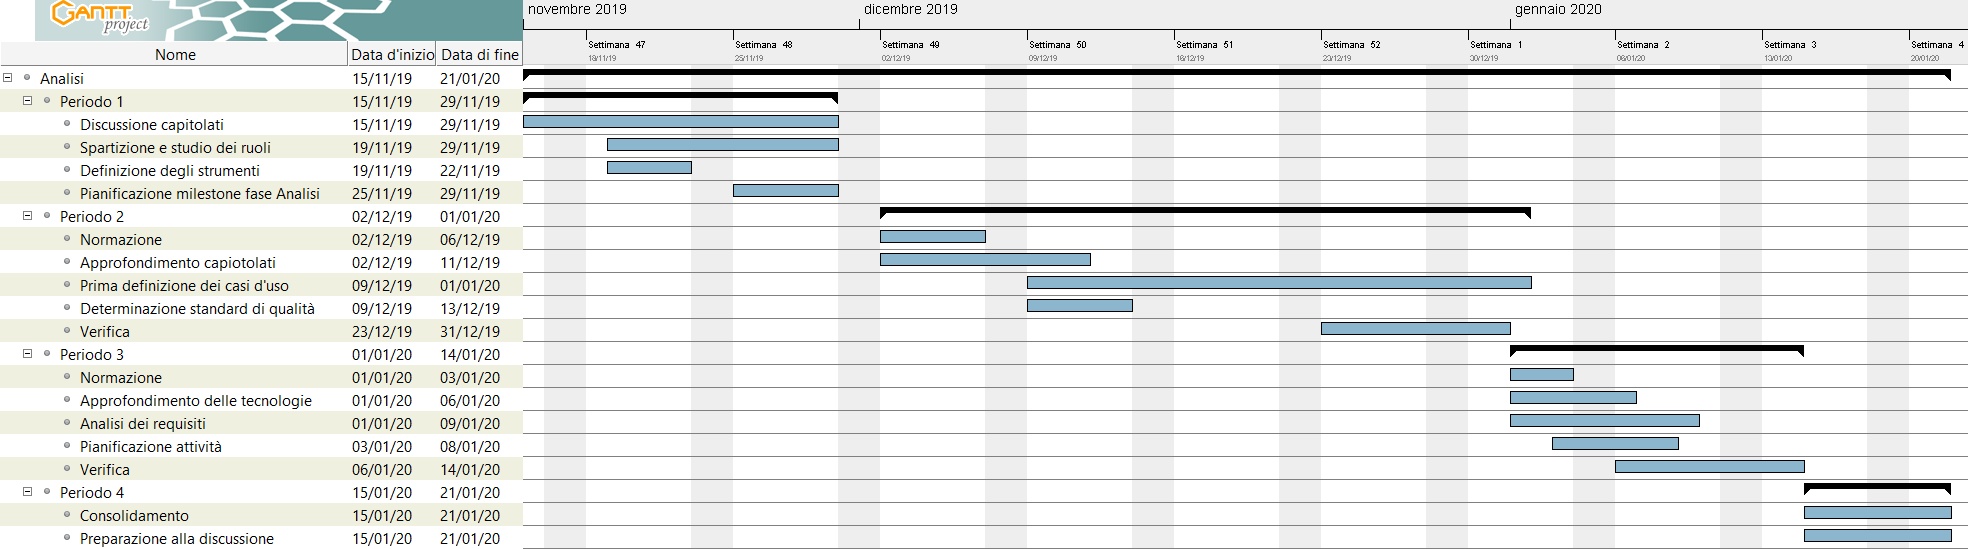
\includegraphics[scale=0.45]{sezioni/DiagrammiGantt/Analisi.png}
	\caption{Diagramma di Gantt delle attività di Analisi}
\end{figure}


\subsection{Progettazione architetturale}
Periodo: dal 2019-01-22 al 2019-03-15.
\\Inizia al termine dell'Analisi dei Requisiti e finisce con la data di consegna della Revisione di Progettazione.
\\In questo macro periodo viene definita una soluzione architetturale in modo da soddisfare i requisiti individuati nel periodo di Analisi dei Requisiti.

\subsubsection{Periodo 1} 
Dal 2019-01-22 al 2019-02-17
\begin{itemize}
	\item \textbf{Normazione:} aggiornamento delle norme;
	\item \textbf{Analisi dei requisiti:} aggiornamento dell'analisi dei requisiti;
	\item \textbf{Pianificazione attività:} aggiornamento della pianificazione delle attività;
	\item \textbf{Standard qualità:} aggiornamento dello standard qualità;
	\item \textbf{Approfondimento sulle tecnologie:} aggiornamento delle tecnologie che si dovranno utilizzare;
	\item \textbf{Verifica};
\end{itemize}
\subsubsection{Periodo 2} 
Dal 2019-02-18 al 2019-03-08
\begin{itemize}
	\item \textbf{Studio delle tecnologie:} IAAS Kubernetes\ap{G} o PaaS\ap{G}, Openshift\ap{G} o Rancher\ap{G}, LDAP\ap{G} e GPS\ap{G};
	\item \textbf{Normazione:} aggiornamento delle norme;
	\item \textbf{Standard qualità:} aggiornamento dello standard qualità;
	\item \textbf{Technology Baseline\ap{G}:} redazione della Technology baseline;
	\item \textbf{Proof of Concept\ap{G}:} rappresentazione della Baseline\ap{G};
	\item \textbf{Codifica:} viene codificato il Proof of Concept;
\end{itemize}
\subsubsection{Periodo 3} 
Dal 2019-03-09 al 2019-03-15
\begin{itemize}
	\item \textbf{Consolidamento};
	\item \textbf{Preparazione per la revisione di Progettazione};
\end{itemize}
\subsubsection{Diagramma di Gantt delle attività}
\begin{figure}[h]
	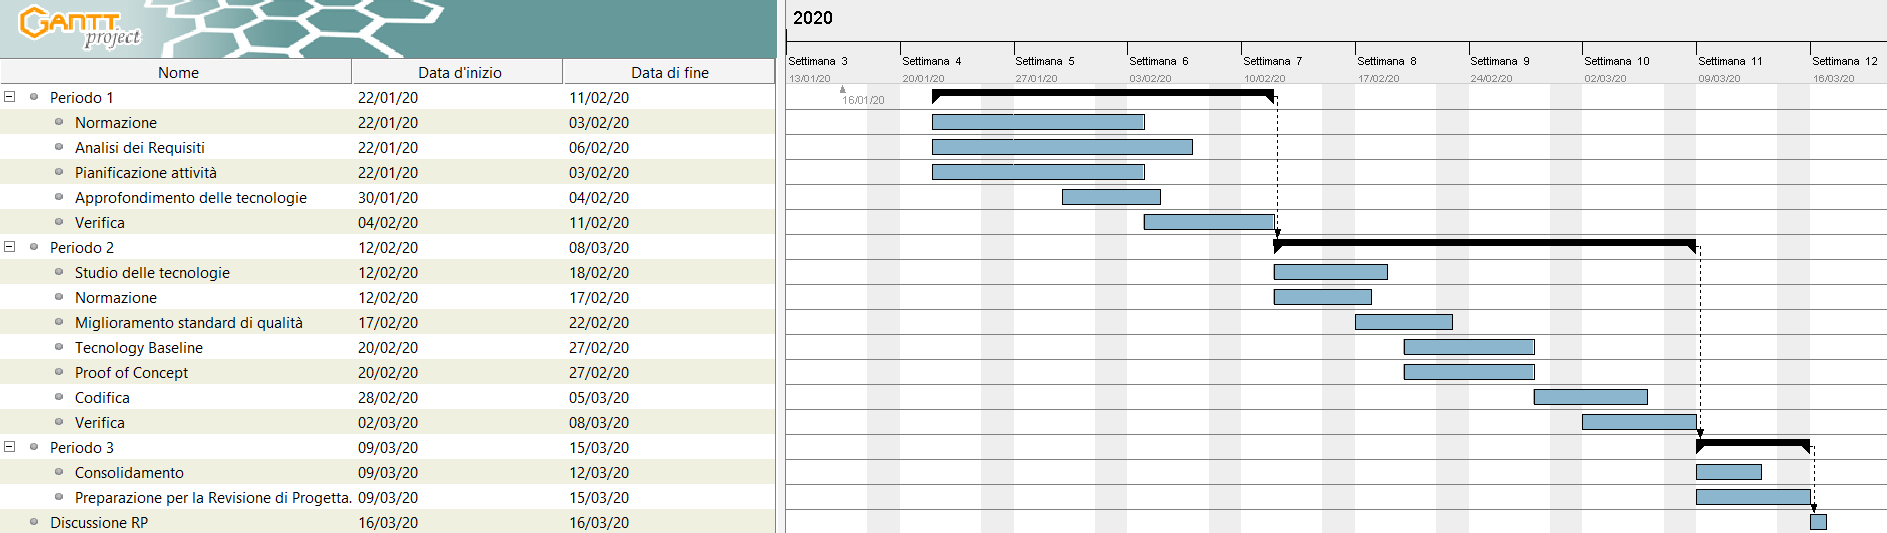
\includegraphics[scale=0.45]{sezioni/DiagrammiGantt/ProgettazioneArchitetturale.png}
	\caption{Diagramma di Gantt delle attività di Progettazione architetturale}
\end{figure}

\subsection{Progettazione di dettaglio e codifica}
Dal 2020-03-16 al 2020-04-19\\

\subsubsection{Periodo 1} 
Dal 2020-03-16 al 2020-03-27\\
\begin{itemize}
	\item \textbf{Approfondimento delle tecnologie};
	\item \textbf{Normazione};
	\item \textbf{Pianificazione delle attività};
	\item \textbf{Progettazione};
	\item \textbf{Codifica :}Implementazione dei requisiti di base identificati per ottenere un sistema stabile;
	\item \textbf{Maunuale utente: }Stesura manuale in relazione alle funzionalità di base del sistema;
\end{itemize}
\subsubsection{Periodo 2} 
Dal 2020-03-28 al 2020-04-08\\
\begin{itemize}
	\item \textbf{Implementazione della Product Baseline :} segueno le specifiche della tecnology baseline;
	\item \textbf{Progettazione};
	\item \textbf{Codifica incrementale: }Aggiunta di requisiti al sistema tramite incrementi;
	\item \textbf{Incremento e verifica :}Verifiche ed eventuali aggiunte al lavoro svolto in precedenza;
	\item \textbf{Manuale utente: }Aggiunta al manuale delle funzionalità inserite incrementalmente nel sistema;
	\item \textbf{Verifica: }Verifica dell'andamento del team in relazione alle tempistiche e allo svolgimento dei compiti assegnati;
\end{itemize}
\subsubsection{Periodo 3}
Dal 2020-04-09 al 2020-04-12\\
\begin{itemize}
	\item \textbf{Primo rilascio prodotto};
	\item \textbf{Stesura lettera di presentazione}.
\end{itemize}
\subsubsection{Periodo 4} 
Dal 2020-04-13 al 2020-04-19\\
\begin{itemize}
	\item \textbf{Stesura presentazione RQ};
	\item \textbf{Studio per la discussione};
\end{itemize}
\subsubsection{Diagramma di Gantt delle attività}
\begin{figure}[h]
%	\includegraphics[scale=0.45]{sezioni/DiagrammiGantt/ }
	\caption{Diagramma di Gantt delle attività di Progettazione di dettaglio e codifica}
\end{figure}


\subsection{Validazione e collaudo}
Inizia al termine della progettazione di dettaglio e codifica e finisce con la data di consegna della Revisione di Accettazione.
\\In questo macro periodo vengono definite le attività che servono per verificare che il prodotto corrisponde a quello desiderato dal cliente.
\subsubsection{Periodo 1} 
Dal 2019-04-21 al 2019-04-30
\begin{itemize}
	\item \textbf{Normazione};
	\item \textbf{Analisi dei requisiti};
	\item \textbf{Pianificazione attività};
	\item \textbf{Rifinitura del prodotto};
\end{itemize}
\subsubsection{Periodo 2} 
Dal 2019-05-01 al 2019-05-10
\begin{itemize}
	\item \textbf{Codifica:} verrà eseguito l'ultimo versionamento del prodotto;
	\item \textbf{Verifica:} verrà accertato che le esecuzioni delle attività siano esenti da errori;
	\item \textbf{Validazione:} verrà verificato se il prodotto realizzato sia conforme alle attese;
	\item \textbf{Scrittura dei manuali:} vengono scritti il manuale Utente e il manuale Manutentore;
	\item \textbf{Collaudo:} vengono eseguiti gli ultimi test sul prodotto per verificare se le funzionalità rispettano i risultati attesi;
\end{itemize}
\subsubsection{Periodo 3} 
Dal 2019-05-11 al 2019-05-17
\begin{itemize}
	\item \textbf{Consolidamento};
	\item \textbf{Preparazione per la revisione di Accettazione};
\end{itemize}
\subsubsection{Diagramma di Gantt delle attività}
\begin{figure}[h]
	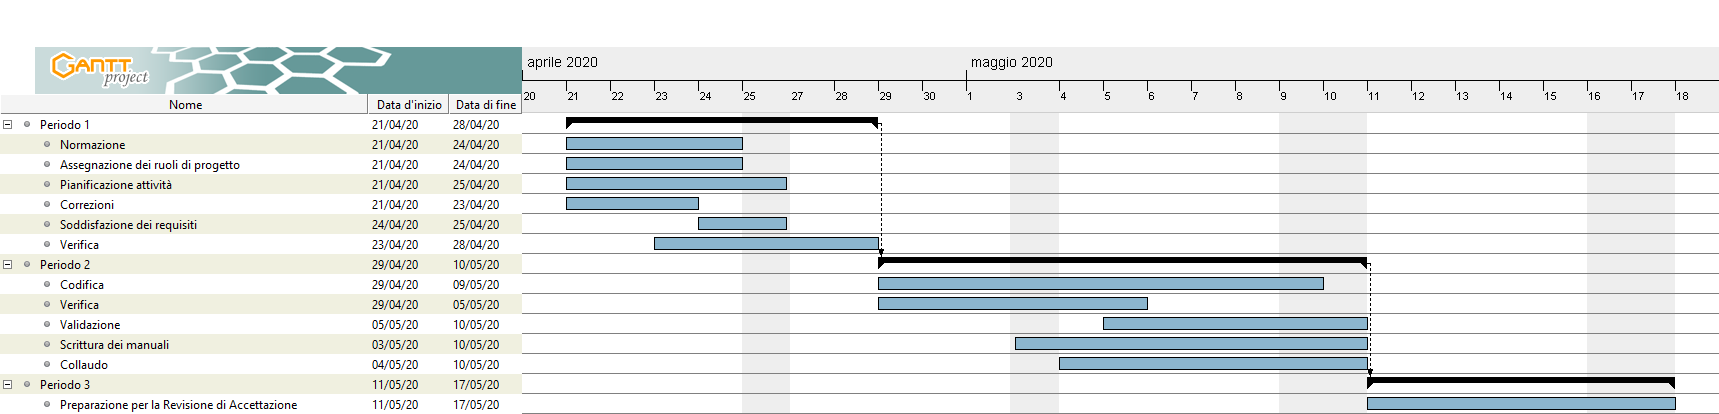
\includegraphics[scale=1.1]{sezioni/DiagrammiGantt/Validazione.png}
	\caption{Diagramma di Gantt delle attività di Validazione e Collaudo}
\end{figure}
